
\begin{table}
\caption{Overview of assimilation experiments performed.}
\centering
\begin{tabular}{p{2cm}p{5cm}p{4cm}}
Experiment number &  Assimilated Quantities  & Run dates \\
\hline
1 &  none	& 1 Jan - 28 Feb 2009 \\
2 &  $\chi_1$, $\chi_2$, $\Delta$LOD		& 1 Jan - 28 Feb 2009 \\
3 &  Radiosonde temperatures	& 1 Jan -31 Jan 2009	\\
4 &  Radiosonde temperatures, $\chi_1$, $\chi_2$, $\Delta$LOD	& 1 Jan - 17 Jan 2009\\
5 & \textcolor{unsure}{CHAMP-like GPS-RO refractivities} & \textcolor{alert}{FILL IN}	\\
\hline
\end{tabular}
%\tablenotetext{a}{Footnote text here.}
\label{tab:expts}
\end{table}

 \begin{figure}
\includegraphics[width=\textwidth]{../../Documents/Plots/ERP_DA/radiosonde_locations.pdf} 
 \caption{  }
 \label{fig:RS}
\end{figure}

 \begin{figure}
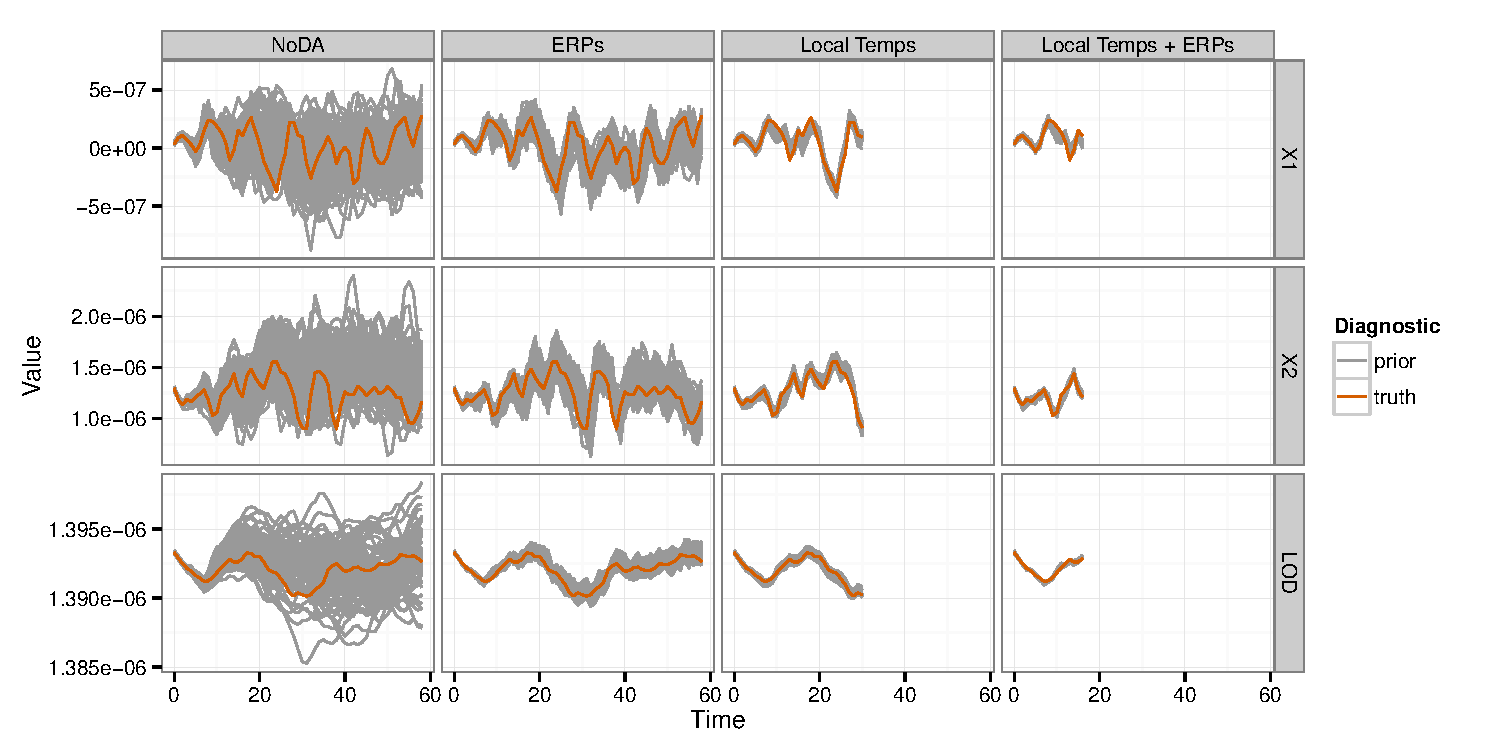
\includegraphics[width=\textwidth]{../../Documents/Plots/ERP_DA/paper/fit_to_ERPs.pdf} 
 \caption{ The DART prior ensemble (gray) compared to the true state (orange) in terms of assimilation time and each of the three angular momentum functions [(\ref{eq:X1})-(\ref{eq:X3}), (\ref{eq:X3_to_LOD})].  The columns compare the four experiments summarized in Table \ref{tab:expts}.  }
 \label{fig:fit_to_ERPs}
\end{figure}

 \begin{figure}
 \includegraphics[width=\textwidth]{/home/lneef/Dropbox/NATHAN/Projects/ERP_DA/Plots/paper_NODAvsERPALL_MSEprofiles_Ulev_time.pdf}
 \caption{First column: mean square error in zonal wind as function of vertical level and time, for the NODA experiment (top), the AAMDA experiment (center), and the difference between the two (bottom). Second column: as in the first column but showing scaled ensemble variance. All quantities are averaged zonally and meridionally.} 
 \label{fig:MSEprofiles}
\end{figure}

 \begin{figure}
 \includegraphics[width=\textwidth]{/home/lneef/Dropbox/NATHAN/Projects/ERP_DA/Plots/paper_NODAvsERPALL_MSEprofiles_Ulat_time.pdf}
 \caption{First column: mean square error in zonal wind as function of latitude and time, for the NODA experiment (top), the AAMDA experiment (center), and the difference between the two (bottom). Second column: as in the first column but showing scaled ensemble variance. All quantities are averaged vertically between 200 and 500 hPa, and meridionally.} 
 \label{fig:MSEsurface}
\end{figure}




 \begin{figure}
 \includegraphics[width=\textwidth]{/home/lneef/Dropbox/NATHAN/Projects/ERP_DA/Plots/paper_RSTvsERPRST_MSEprofiles_Ulev_time.pdf}
 \caption{As in Fig. \ref{fig:MSEprofiles}, but not now comparing experiments RST and AAMRST.}
 \label{fig:MSEprofiles2}
\end{figure}

 \begin{figure}
 \includegraphics[width=\textwidth]{/home/lneef/Dropbox/NATHAN/Projects/ERP_DA/Plots/paper_RSTvsERPRST_MSEprofiles_Ulat_time.pdf}
 \caption{As in Fig. \ref{fig:MSEsurface}, not now comparing experiments RST and AAMRST.}
 \label{fig:MSEsurface2}
\end{figure}

\begin{figure}
	\includegraphics[width=0.8\textwidth]{/home/lneef/Dropbox/NATHAN/Projects/ERP_DA/Plots/paper_RH.pdf}
 \caption{Rank histograms for the zonal wind for the four main experiments, computed at 3-day integrals over the first 17 days of assimilation.}
 \label{fig:RHprogression}
\end{figure}


